\documentclass{article}
\usepackage{german}
\usepackage[latin1]{inputenc}
\usepackage{a4wide}
\usepackage{amssymb}
\usepackage{fancyhdr}
\usepackage{fancyvrb}
\usepackage{alltt}
\usepackage{epsfig}
\usepackage{hyperref}
\pagestyle{fancy}
\usepackage{lastpage}

\fancyfoot[C]{--- \thepage/\pageref{LastPage}\ ---}

\hypersetup{
	colorlinks = true, % comment this to make xdvi work
	linkcolor  = blue,
	citecolor  = red,
        filecolor  = blue,
        urlcolor   = [rgb]{0.5, 0.4, 0.0},
	pdfborder  = {0 0 0} 
}


\renewcommand*{\familydefault}{\sfdefault}

\pagestyle{fancy}

\renewcommand{\labelenumi}{(\alph{enumi})}
\renewcommand{\labelenumii}{\arabic{enumii}.}

\begin{document}
\noindent
{\Large \textbf{Aufgaben-Blatt}: Ein Rangier-Problem}
\vspace{0.5cm}


\noindent
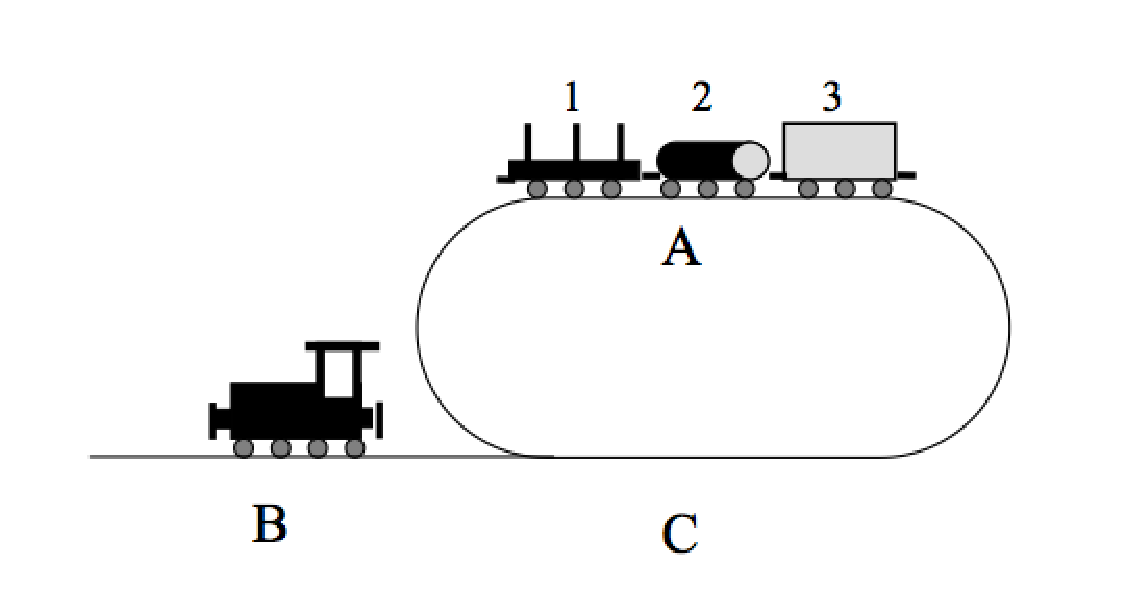
\epsfig{file=rangierProblem, scale=0.8}

\noindent
Auf dem Gleis-Abschnitt A befinden sich drei Waggons, die wir mit 1, 2, 3
bezeichnen.  Auf dem Gleisabschnitt B befindet sich eine Lokomotive, die wir sp�ter mit der
Ziffer 0 bezeichnen.   Ziel ist es, die
Waggons in der Reihenfolge 3, 1, 2 auf dem Gleis-Abschnitt C abzustellen.  Die Lokomotive
soll am Schluss wieder auf den Gleis-Abschnitt B zur�ckfahren.  Die Lokomotive kann die Waggons in
beliebiger Reihenfolge an und abkoppeln.  Beim Rangieren ist es erlaubt, dass die
Lokomotive gleichzeitig Waggons vorne und hinten anh�ngt.

Schreiben Sie ein \textsc{SetlX}-Programm, dass die gestellte Aufgabe l�st.  
Laden Sie dazu von meiner Seite das Programm
\\[0.2cm]
\hspace*{-0.8cm}
\href{https://github.com/karlstroetmann/Logik/blob/master/Aufgaben/Blatt-5/shunting-frame.stlx}{\texttt{https://github.com/karlstroetmann/Logik/blob/master/Aufgaben/Blatt-5/shunting-frame.stlx}} 
\\[0.2cm]
herunter und bearbeiten Sie die folgenden Teilaufgaben.
\begin{enumerate}
\item Definieren Sie in Zeile 69 eine Funktion \texttt{toList} so, dass f�r eine Menge
      $s$ der Aufruf $\textsl{toList}(s)$ die Menge aller Listen berechnet, deren Elemente
      aus $s$ sind und die jedes Element aus $s$ genau einmal enthalten.  Beispielsweise
      soll der Aufruf $\mathtt{toList}(\{1,2,3\})$ das Ergebnis
      \\[0.2cm]
      \hspace*{1.3cm}
      $\{[1, 2, 3], [1, 3, 2], [2, 1, 3], [2, 3, 1], [3, 1, 2], [3, 2, 1]\}$
      \\[0.2cm]
      liefern.
\item Definieren Sie in Zeile 79 eine Prozedur \texttt{inverse} so, dass der Aufruf
      $\mathtt{inverse}(R)$ f�r eine bin�re Relation $R$ die Relation $R^{-1}$ berechnet.
      Beispielsweise soll gelten:
      \begin{verbatim}
      inverse({ ["a", 1], ["b", 2] }) = {[1, "a"], [2, "b"]}.
      \end{verbatim}
\item Wir stellen die Waggons durch die Ziffern 1, 2 und 3 dar, die Lokomotive wird durch
      0 dargestellt.

      Definieren Sie in Zeile 91 die Menge \texttt{partitions} so, dass diese Menge alle
      Tripel der Form
      \\[0.2cm]
      \hspace*{1.3cm}
      $\langle a, b, c \rangle$
      \\[0.2cm]
      enth�lt, f�r welche die Menge $\{ a, b, c \}$ eine Partition der Menge $\{0,1,2,3\}$
      ist.

      \textbf{Hinweis}:  Die Menge $\{0,1,2,3\}$ hat 81 Partitionen, die aus drei Mengen bestehen.
\pagebreak
\item Wir stellen Situationen durch Listen der Form
      \\[0.2cm]
      \hspace*{1.3cm}
      $[ la, lb, lc ]$
      \\[0.2cm]
      dar.  Dabei ist $la$ die Liste der Waggons auf dem Gleis A, $lb$ ist die Liste der
      Waggons auf dem Gleis $B$ und $lc$ ist die Liste der Waggons auf dem Gleis C.
      
      Berechnen Sie in Zeile 98 die Menge aller Situationen.

      \textbf{Hinweis}:  Es gibt 360 verschiedene Situationen.
\item Berechnen Sie in Zeile 111 die Menge aller Transitionen, in denen die Lokomotive vom
      Gleis A nach Osten zum Gleis C f�hrt.

      \textbf{Hinweis}:
      Es gibt in \textsc{SetlX} eine Funktion \texttt{reverse}, die eine Liste umdreht.

      \textbf{Hinweis}: Es gibt hier 210 verschiedene Transitionen.
\item Berechnen Sie in Zeile 126 die Menge aller Transitionen, in denen die Lokomotive vom
      Gleis A nach Westen zum Gleis C f�hrt.

      \textbf{Hinweis}: Hier gibt es ebenfalls 210 verschiedene Transitionen.
\item Berechnen Sie in Zeile 140 die Menge aller Transitionen, in denen die Lokomotive vom
      Gleis C zum Gleis A f�hrt.  Ber�cksichtigen Sie dabei die Symmetrie des Problems.
\item Berechnen Sie in Zeile 144 die Menge aller Transitionen, in denen die Lokomotive vom
      Gleis B zum Gleis C f�hrt.
\item Berechnen Sie in Zeile 156 die Menge aller Transitionen, in denen die Lokomotive vom
      Gleis C zum Gleis B f�hrt.

      \textbf{Hinweis}: Die Relation, die alle m�glichen Transitionen enth�lt, hat 1140 verschiedene
      Elemente. 
\end{enumerate}
\textbf{Hinweis}:  Der Pfad, der am Ende berechnet wird, hat die L�nge 13.

\end{document}

%%% Local Variables: 
%%% mode: latex
%%% TeX-master: t
%%% End: 
